\chapter{Methods}
\label{sec:methods}

%Several domains of application of biological sciences and computer sciences are recognized, such as Medical informatics %(MI)\nomenclature{MI}{Medical informatics} 
%which deals with informatics methods used in clinical medicine and healthcare. Bioinformatics %(BI)\nomenclature{BI}{Bioinformatics} 
%focus more on development and application of new informatics techniques in biological (mainly genomic) sciences. Computational Biology % (CB)\nomenclature{CB}{Computational biology}
%study the biological systems with methods involving mathematical models, computational simulation techniques. Recent development in the medical informatics, bioinformatics and other disciplines joined a scientific effort to translate the successful techniques into clinical medicine and healthcare and vice-versa and Maojo et al. \cite{Maojo2003} and Martin-Sanchez et al.\cite{Martin-Sanchez2004} described relationship between medical informatics and bioinformatics to determine a new domain of biomedical informatics.

%Further chapters touch the approach to develop new techniques in informatics inspired from genetic and biology and deliver such techniques to clinical use or basic research within the field of computational biology.

The general issue of utilizing grid or cloud computing infrastructures is the selection of the appropriate method that is used to integrate domain-specific computations into the grid or cloud infrastructure of a concrete provider. 

Various tools are already available within current grid infrastructures, including open-source and licensed software for computation. The local scientific grid provider may give a list of the available applications\footnote{applications available in CESNET METACENTRUM \url{https://wiki.metacentrum.cz/wiki/Kategorie:Applications} accessed February 2015}. Alternatively, application databases are available in a broader environment, e.g., in the EGI.eu application database\footnote{\url{https://appdb.egi.eu/} accessed February 2015}.
Additionally, the workflow systems and scientific gateways that are mentioned in section \ref{sec:introworkflow} try to hide the complexity of grid or cloud computing infrastructures and may also be used to integrate specific domains.
In designing a new application, the programming model of parallel computing and/or distributed  computing (in section \ref{sec:parallelprogramming} and  \ref{sec:distributedprogramming}) needs to be followed, utilizing the benefits of grid computing and cloud computing.

The general approach to port applications to a grid infrastructure is to automatize what can be automatized, i.e., make scripts, configure system, prepare some user interface, integrate with existing applications, utilize protocol compatibility, etc. Additionally, the prepared template, script or application should be reused for further similar computational requests.
%Efforts to obtain the first results are high, however, if the prepared template, script or application is reused for further computational requests, then the effort is much lower.  

\section{Sharing Medical Images}
\label{sec:imaging}
%\label{sec:medicalapp}
%Acquiring, storing and processing digital medical images 
%This chapter introduces acquiring, storing and sharing digital medical images and related metadata within hospital or healthcare provider and among them and research institution.

%are covered in section \ref{sec:introimages}. Overview of analysis of speech and voice and it's relation to voice science is in section \ref{sec:introvoice}. Overview of models and simulation of human physiology and it's relation to systems biology is briefly covered in section \ref{sec:intromodels}.


%The computing in biomedicine can be divided into research and clinical application. %Translational science aims to "translate" findings from research to better health care including diagnostic tools, procedures, drugs, etc.

%In case of research use-cases, processing medical information helps to make more precise current theories or support formulating new one. In case of clinical use cases, processing medical information helps to analyse and interpret the information, predicting future trends and support decision on some intervention.

%\footnote{Motivation of using distributed computing technologies is to share physical data, among multiple organizations, where there is no need or other barriers to store all data centrally, e.g. for legal or capacity limitation. A lot of medical information within biomedical research came from real patient and such information are protected by some regulation and processing of them is regulated and controlled by the country laws or international agreements. Thus there must be considered ethical as well as legal issues how to deal with such information. Sharing and processing of medical images are covered in section \ref{sec:introimages}. Providing access to services with high values is another motivation of using distributed computing technologies. E.g. basic and advanced analysis of biological signals, especially of voice is described in section \ref{sec:introvoice}.}


Use cases that relate to digital medical images involve image acquisition, preprocessing, storing and searching.
Clinicians mainly use patient images for visualization and diagnostic purposes. Computer assisted methods facilitate the diagnostic process and involves image enhancement (to reduce the image noise and to increase the contrast), image segmentation (to separate different types of structures from the background and from each other), quantification methods (to determine the structure shape, size and volume) and registration methods (to process and join multiple different images into one).
Comprehensive concepts and digital techniques in medical imaging are presented in published works edited by I.N.Bankman\cite{Bankman2000}.

The acquisition of a medical image is performed with different modalities (different types of equipment and sensors) by radiologists or other specialists. The DICOM\footnote{DICOM: \url{http://dicom.nema.org/} accessed January 2015}\nomenclature{DICOM}{Digital Imaging and Communication Protocol} format and protocol has become an industrial standard for exchanging medical images electronically and in Picture Archiving Communication Systems (PACS). PACS holds the acquired DICOM images with metadata and description, which are  noted by experts. PACS is usually part of the information systems in hospitals. Figure \ref{fig:pacs} shows the typical workflows of a medical image in a hospital.

\begin{figure}[ht]
    \centering
    \includegraphics[width=0.8\textwidth, height=8cm]{img/chapter3-pacs.png}
    \caption{The typical workflow of a medical image in a hospital. Data acquisition is made by modalities (magnetic resonance, ultrasonography, X-ray radiography, etc.). By using the DICOM format and protocol, it can be directly transferred and visualized by diagnostic workstation. With the metadata filled by an expert physician, the image is stored in PACS. Other desktops within the hospital can retrieve the image and review the report. The hospital information system may be involved in other workflows and communicate with other formats and standards (e.g., HL7).
    }
    \label{fig:pacs}
\end{figure}

As the data that are processed in hospital information systems contains sensitive information of real patients, they are protected  and manipulation with such data are regulated per national or international laws or agreements. The development of telecommunication and network technologies has enabled telemedicine -- providing healthcare over a remote distance. This  requires the sharing and exchanging of sensitive data of real patients among different healthcare providers and such data may be very valuable for further research. Security and encryption should be addressed, because the DICOM standard itself does not appropriately solve security issues. Thus, encryption during the transferring of data over to a computer network must be ensured.
%%% 2 April correction ---
In the Czech Republic, there are several projects in production that interconnect different hospitals, clinics and other healthcare organizations in order to exchange medical images. Project ePACS allows the interconnection of each participant's PACS system via a dedicated Virtual Private Network (VPN)\nomenclature{VPN}{Virtual Private Network} channel to the central node. The exchange of medical images is realized via DICOM protocol by routing the communication from one VPN channel to the other\footnote{ePACS:\url{http://www.epacs.cz}, accessed January 2015}. Another approach is used in the project MEDIMED, which is held by Masaryk University in Brno. Instead of a dedicated VPN channel, they use Secure Sockets Layer (SSL)\nomenclature{SSL}{Secure Sockets Layer} encryption over the standard DICOM protocol going on top of TCP/IP communication. Regional hospitals and healthcare providers are interconnected via the MEDIMED servers, as presented by Slavicek et al. \cite{Slavicek2010}.% \cite{Javornik2011,Zatloukal2012}.
In other countries, cross-border teleradiology was tested in projects of Baltic e-health, R-Bay and others, which were published by Ross et al. \cite{Ross2010} and Saliba et al. \cite{Saliba2012}.
These projects focused on the sharing of medical images, as well as other knowledge and information.

Access to a wide range of medical images is needed for the research of new processing and diagnostic methods, rare diseases, developing new detection algorithm, etc.  DICOM records are "de-identified" (identification of patient records are deleted and only the date of bird and other non-personal data are kept) or anonymized (additional information is manipulated to prevent potential disclosure) in order to protect sensitive personal data, but keep important information for research purposes. The Globus MEDICUS project, published by Erberich et al. \cite{Erberich2006,Erberich2007}, is based on Globus Toolkit middleware in order to federate clinical and research application via a grid computing infrastructure. The project has been in hibernation since 2008 and no further development has been published\footnote{\url{https://dev.globus.org/wiki/Incubator/MEDICUS} accessed February 2015}. Similar efforts were made by the Medical Data Manager project, which used gLite grid middleware deployed within european grid infrastructure EGEE (predecesor of EGI) and was published by Duque, Montagnat et al.\cite{Duque,Montagnat2007} \footnote{\url{http://modalis.i3s.unice.fr/softwares/mdm/start} accessed February 2015}. The MediGRID project, which was published by Krefting et al.\cite{Krefting2009}, added additional processing of images within selected use cases that are supported by a grid computing infrastructure \cite{Krefting2010}. The Health-e-Child project aimed to interconnect research institutions and hospitals in United Kingdom, France and Italy for the purpose of a grid-based healthcare platform for pediatric health-care \cite{Skaburskas2008}. The Neurist project developed system, connecting  clinicians and researchers in order to improve research and the treatment of cerebral aneurysm. This provided the tools to analyze and interpret patient data and gave researchers access to a set of aneurysm data, published by Benkner et al.\cite{Benkner2010}.
The SEAGRIN research project aimed to share knowledge, mainly for educational purposes, in semi-formally described semantics. Kuba et al. published this proposal and its implementation \cite{Kuba2006}. 

The storing of sensitive medical information, which is even de-identified or anonymized, is usually restricted. This led to the idea of storing such information within trusted institutions, e.g., hospitals, and to move and facilitate the deployment of grid services that store medical data to that institution. For example, pre-installed virtual machines can contain grid services and are deployed as a sealed grid, as proposed by Kuba et al.\cite{Kuba2007a}.


%When we look to the architecture of the systems of sharing medical images the problematic part within the point-to-multipoint architecture is the central part of the systems already in production e.g. in Czech Republic (MEDIMED, ePACS). This may become single point of failure and bottleneck.

To summarize this section, in past years, digital medical image acquisition, storing, exchanging and processing has become common and it currently uses distributed computing techniques. Several efforts have been made to implement medical data management within grid or cloud infrastructures for research purposes and to integrate them with production infrastructures. Security is solved by authentication and authorization mechanisms, as well as by encrypting data and/or de-identification or anonymization but keeping minimal information that is required for research purposes. A related question is how easily the previously mentioned grid-based technologies can be integrated with current systems in hospitals or institutions that main purpose is common health-care. The following section describes selected methods that are used to integrate a pilot deployment of Globus MEDICUS with the current regional system for exchanging medical images - MEDIMED.

\subsection{Methods to share medical images in grid}
\label{sec:methodsimages}

The Globus toolkit belongs to a group of the most used grid middleware (see section~\ref{sec:servicegrid}). The core service included in Globus Toolkit is GridFTP -- grid extension to file transfer protocol(FTP)\nomenclature{FTP}{File Transfer Protocol}. This implements strategies such as \emph{stripping data} into multiple pieces; the \emph{parallel transfer of data}, utilizing stripped data parts to be transferred via different channels; \emph{partial file transfer}, some applications may not need to access the whole file but rather a smaller portion of it, etc., as described by Foster et al. and Allcock et al. \cite{Foster2006, Allcock2005}. Other core services are Replica Location Service, which aims to localize data, and Globus Resource Allocation Management (GRAM), which provides web service and proxies to the lower level job scheduler's implementation \cite{Foster2006}.

Next to core services, the domain-specific services might be implemented for the purpose of an application that uses the Open Grid Service Architecture (OGSA). Globus MEDICUS \cite{Erberich2006,Erberich2007} implements a DICOM Grid Interface Service (DGIS) and integrates the open-source PixelMed\texttrademark ~Java DICOM Toolkit\footnote{\url{http://www.pixelmed.com/} accessed February 2015} into a web service, communicating via the DICOM protocol. Furthermore, it forwards queries to the underlying services within Globus toolkit. 

DGIS acts as a gateway to a grid infrastructure. As communication via the DICOM protocol is not secured, it is recommended that the DGIS be installed on the location of the PACS system or the DICOM ready modality or software. When a DICOM study is uploaded into DGIS, it is anonymized and stored. A record is made into another service’s Meta Catalog service, which resides in the same domain or anywhere in the grid that is accessible via the Globus Toolkit. Such an anonymized database of DICOM records can be used to query via the DGIS interface and to, for example, integrate with web-based applications, showing records for research purposes. Furthermore, authentication and authorization can be achieved in this level. 
To integrate this system with an existing system MEDIMED project \cite{Slavicek2010} for sharing the medical images, the special client software "RediMed console", needs to be installed next to the DGIS. DGIS behaves as an access point to a PACS system whose records can be exchanged via the RediMed console software to other MEDIMED participants. 
The results of this particular deployment and integration are presented in section \ref{sec:resultsimages}.
%The software for processing medical images can retrieve them from DGIS via DICOM protocol. 

%To present DICOM studies The integration strategy based on shared database or files can be used to present the DICOM studies via web portal. Additionally the web portal might generate specific DICOM queries to DGIS.


%The following section will cover methods related to the integration effort.

%The section~\ref{sec:introintegration} describes several general software architectural styles and integration patterns used in further in this work. 
%The section~\ref{sec:methodsimages} describes specific methods used in the area of processing  medical images within grid infrastructure to verify the integration effort between research and hospitals systems. The section~\ref{sec:methodsvoice} describes a method to deploy existing application as a service to the distributed infrastructure.The section~\ref{sec:methodsmodels} focus on modelling methodology in order to build and maintain complex models of human physiology as the complex models seems to mainly benefit from parallel computation. And the subsection~\ref{sec:methodsmodelsestimate} follows up on the modeling methodology to describe the system for estimating model parameters. 

%as a program to start within remote session and , the interactive application allows select type of voice which will be analysed. After recording is finished, the whole recording is analyzed with FFT to obtain full spectral analysis. 

%\section{Integrating heterogenous systems}
%\label{sec:introintegration}
%
%Integrating heterogenous system into a well designed enterprise application has some issues which needs to be addressed.
%
%One of the first decision which may be hard to change in future is platform. Platform might be determined by third party platform-specific product incorporated in a workflow which cannot be changed. There exists software platforms that may run on different operating systems. E.g. Java platform is based on the idea that a program is compiled into bytecode which is then interpretted by just-in time compilers on target platform. Similar approach applies to Common Language Infrastructure (CLI) known by it's implementation .NET Framework on Microsoft Windows operating system or MONO which is implemented on Linux platforms.
%Another approach to address the issue of a platform is virtualization as mentioned already in section \ref{sec:introvirtual}.
%
%
%%\subsection{File exchange}
%Is based on the fact, that one process produces a file which is consumed by another process. This is popular in batch processing systems which needs no or only limited interactivity with user. The grid workflow management systems 
%\subsection{Message Oriented Integration}
%The processes that run concurently synchronize and exchange messages via some dedicated channel. E.g. platform depended
%
%\subsection{Service Oriented Architecture}
%\label{sec:methodssoa}
%Service oriented architecture (SOA) decouples a service contract with intention to be platform independent from it's platform-dependent implementation\cite{Erl2008}. The loosely coupled modules conforming the SOA style are realized as web service which contracts are described in Web Service Definition Language (WSDL) which defines the service interface in term of endpoint location (URL), sset of operation, binding of operation to endpoint, the format of input and output messages and binding of the messages to the operations. These are usually based on some XML dialect. Even the WSDL can be written by hand, it can be generated by a service stack framework for the concrete service implementation. 
%Next to the service implementation there are abstraction like registry and repository holding metadata of the service, so it can be dynamically discovered.
%
%\subsection{RESTful web services}
%\label{sec:methodsrest}
%The Representational State Transfer (REST) architectural style proposed by R. Fielding\cite{fielding2000chapter} is used for representing functionality as a limited  for solving demand issues of the selected tasks 
%

%The images produced by medical devices are mainly in a DICOM standard which describes the file format and communication protocol for exchange, query/retrieve image, modality and other metadata \cite{dicom2011}. The file format consist of header which involves information about the patient and the pixel data containing uncompressed or compressed bitmap of image. Some devices produces multi-frame multi-dimensional images which can be stored in one DICOM file. The DICOM standard is used to interconnect multiple medical devices, local computers and database system which is usually termed as Picture Archiving and Communitation System (PACS). 


%The particular methods used within specific biomedical domains are covered in further chapter section \ref{sec:methodsimages}, \ref{sec:methodsvoice}, \ref{sec:methodsmodels}. 

%This chapter covers general methods which might be utilized in any domain. The section~\ref{sec:introintegration} describes several general software architectural styles and integration patterns and section~\ref{sec:introvirtual} covers virtualization technology.


%The section~\ref{sec:introintegration} describes several general software architectural styles and integration patterns used in further in this work. 
%The section~\ref{sec:methodsimages} describes specific methods used in the area of processing  medical images within grid infrastructure to verify the integration effort between research and hospitals systems. The section~\ref{sec:methodsvoice} describes a method to deploy existing application as a service to the distributed infrastructure.The section~\ref{sec:methodsmodels} focus on modelling methodology in order to build and maintain complex models of human physiology as the complex models seems to mainly benefit from parallel computation. And the subsection~\ref{sec:methodsmodelsestimate} follows up on the modeling methodology to describe the system for estimating model parameters. 


%\begin{itemize}
%\item{ 
%The \emph{Service Oriented Architecture} (SOA) is high level programming model based on self contained units of functionality and metadata, so the service can be dynamically discovered and used. An important aspect is separated service implementation from it's contract or interface \cite{Erl2008} and is usually realized by web services. %More about SOA is in section \ref{sec:methodssoa}.
%}
%\item{
%The \emph{Representation State Transfer} (REST) specifies several architectural constraints that helps scalability, performance and presents functionality via fixed number of operation and uniform resource location \cite{fielding2000chapter}. %More about RESTful web services is in section \ref{sec:methodsrest}
%}
%\end{itemize}
%
%Software architecture of the distributed systems are studied and some repeating patterns are cataloged e.g. by Fowler et. al\cite{Fowler2003}. Integration patterns are discussed with focus on the ways of connecting heterogenous parts of the system as presents Hohpe et al.\cite{Hohpe2002}.

\section{Voice Science}
\label{sec:voice}
With the introduction of objective data analysis and laryngoscopy methods, voice science emphasized the cooperation among laryngologists, speech pathologists and voice teachers.
The normal human voice ranges from 50 Hz to about 1~000 Hz and there are some  individual variations. For the analysis of a digitally recorded voice, either habitual or singing, the Discrete Fourier Transformation (DFT)\nomenclature{DFT}{Discrete Fourier Transformation} is used to produce a frequency and amplitude analysis of the recorded input voice samples. One of the most used class algorithm to compute DFT is the class of Fast Fourier Transformation (FFT)\nomenclature{FFT}{Fast Fourier Transformation} with computational complexity $O(n \log(n))$ \cite{Cooley1965,Frigo2005}.
% and parallel version of the algorithms may introduce additional speedup for larger samples of analyzed data \cite{Gupta1993,Takahashi2003}. 
The result of the analysis can be visualized in a voice range profile (VRP)\nomenclature{VRP}{Voice Range Profile} and the significant difference between an untrained and trained voice can be seen, as published, e.g., by LeBorgne and Weinrich showing a significant difference of VRP after nine-month training \cite{DeLeoLeBorgne2002}. Furthermore, some disorders can be quantitatively seen, which were published, e.g., by Wuyts et al.\cite{wuyts2003effects}.

Another method that is used to analyze vocal chords is laryngoscopy. The videostroboscopy and high speed video in laryngoscope methods produce videos showing real movement of vocal chords. The videokymography method, introduced by Švec et al., complements the videostroboscopy. It allows the visualizing and analyzes of the movement of vocal cords. These movements are recorded by a high speed camera and a new image, constructed from selected line of recorded video, is shown on standard TV or monitor using low frequency \cite{Svec1996,Svec2007}. 

In the case of a recorded sound and further analysis, there is a question about how such a service can be integrated in a grid computing or cloud computing environment in order to provide access to a complex application for non-technical voice specialists. Additionally, analytical software was already developed and calibrated for selected types of microphones in the MS Windows platform by Frič et al. \cite{Fric2007,Fric2012}. Therefore, it was proposed and implemented a method that provides remote access to the analytical software. Section \ref{sec:methodsvoice} describes how the analytical software was customized with a remote desktop protocol (RDP)\nomenclature{RDP}{Remote Desktop Protocol}. Results are described in section \ref{sec:resultsvoice}. A similar approach can be used for processing  video recordings from a laryngoscope, however, the practical limits are discussed in section \ref{sec:conclusion}. 

\subsection{Methods for Remote Analysis of the Human Voice}
\label{sec:methodsvoice}
Terminal access to some remote computational capabilities, e.g., remote command-line or remote execution, is another integration strategy that is used for some remote infrastructures. Secure Shell (SSH) is used to establish a secure channel via an unsecured network (e.g., the Internet) from an SSH client to a SSH server. This is a basic method that is used to access a grid computing infrastructure. 
Remote Desktop Protocol (RDP) is a proprietary protocol that is used for desktop sharing. It was primarily developed in a Microsoft Windows platform, however, today, clients and servers exist for several other platforms. 
%Next to remote command-line, remote execution allows the accessing of remote graphical desktop environments. 

The software for parameterized Voice Range Profile (ParVRP) and Voice Range Profile in Real time (RealVoiceLab) was already developed and calibrated for selected types of microphones in an MS Windows platform by Fric et al. \cite{Fric2007,Fric2012}. Its implementation is carried out in an MATLAB environment, utilizing Signal Processing Toolbox\footnote{\url{http://www.mathworks.com/products/signal/} accessed February 2015}. It is compiled with a MATLAB Compiler and distributed as an executable.

Instead of migrating the application into some compatible platform for grid middleware, a virtual machine was introduced and access to the software was provided via a RDP protocol. RDP itself contains the redirection of several services, e.g., sound recording or drive access. As the default sound recording redirection introduces some sound degradation without control, I proposed, implemented and integrated a custom RDP plugin with the ParVRP and RealVoiceLab software in order to redirect the sound recording without the loss of information. The technical details are in Appendix~\ref{app:remote}. 

The computation of frequencies and amplitude from the recorded samples utilizes the effective Fast Fourier Transformation, which has time complexity $O(n\log(n))$. The benefit of deploying such an application in distributed infrastructures is the immediate access to updated software. Additionally, a collection of anonymized records of voice samples and results are very useful for further research and education. The possible disadvantage is the need to access to Internet.

This type of application can be packaged as a virtual machine template and configured within different types of cloud infrastructures. Together with a script or web portal, the on-demand deployment can be automated. The client part (RDP client) needs to connect to the appropriate instance. The results of such a deployment are discussed in section~\ref{sec:resultsvoice}.

\section{Computational physiology}
\label{sec:models}
A mathematical formalization of the fundamental knowledge and relation among a biological system – a mathematical model - is used as a base abstraction in order to utilize the current discoveries of the genomics and proteomics. It is also used to formalize the knowledge and construct a "Physiome Model". By  definition, a model is the simplification of a complex reality.

Constructing the models and integrating them into a complex entity, which can be used for further purposes, is schematically illustrated in Figure \ref{fig:modeling}. The measurements are carried out in laboratories or in hospitals. Lumped parameter models are usually represented as ordinary differential equations and differential algebraic equations. They characterize the reality as a topology of discrete elements. The imaging methods for processing and analysis (section \ref{sec:imaging}) are used to construct 3D models from segmentation and generate mesh representations that are connected to physical principles. 
\begin{figure}[ht]
    \centering
    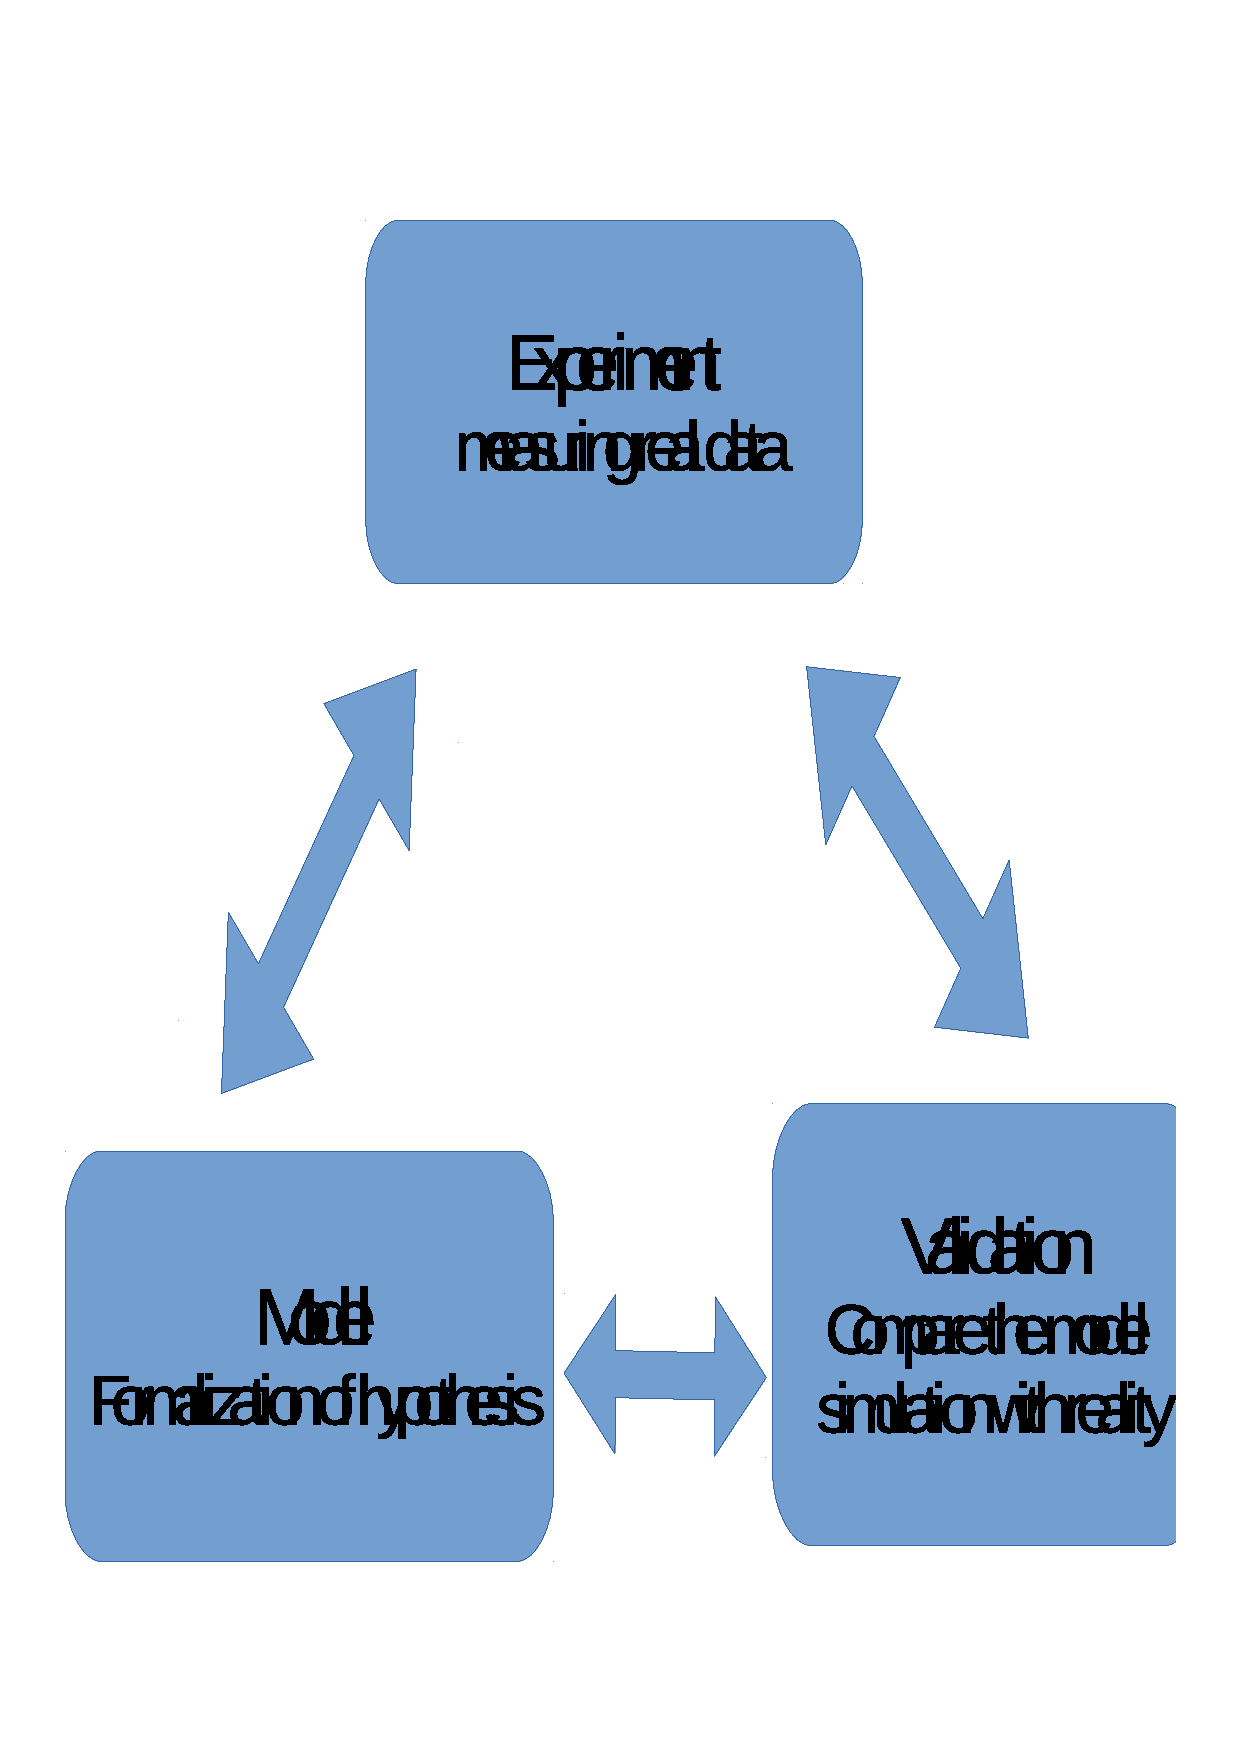
\includegraphics[width=1\textwidth]{chapter3/modeling.png}
    \caption{Schematic illustration of the scientific process. The experiments produce data that are interpreted and a hypothesis is formalized as a model. Validation compares the model simulation with the experiment, if the model satisfies the criteria - if it is in agreement with real experiments, then the validated model can be used for other purposes. %\bibentry{EGICompendium2013} \bibentry{egi2014}.
    }
    \label{fig:modeling}
\end{figure}

The application of mathematical modeling techniques towards biomedical research is sometimes called systems biology. This approach combines the reductionism and integration, as denoted by Kohl et al.\cite{Kohl2010}. Application towards clinical practice includes the quantification of the diagnostic index or treatment strategy. It is a goal to develop tools, database models and methods of several Physiome projects, e.g., VPH-Physiome project presented by Hunter et al.\cite{Hunter2009}.

One of the earliest complex and integrative modeling efforts was a model of circulation and its regulation, which was published by Guyton et al. in 1972 \cite{Guyton1972}. It continues as a "Human Model" or "HumMod" via derivative and technological upgrades, as introduced by Hester et al. \cite{Hester2011systems,hester2011}, with a focus on integration efforts. A different approach of modeling the human physiology is to construct a database of smaller models, which focus on some particular physiological phenomenon. For example, the NSR Physiome project introduces a  JSIM\footnote{JSIM: \url{http://www.physiome.org/jsim/} accessed January 2015} Java-based simulation system in order to support modeling in  physiology. A repository of several hundred models was published using this system \cite{Butterworth2014}. A similar effort is made by the IUPS Physiome project and repositories of the models are  based on XML standard languages CellML and FieldML \cite{Hunter2004,Yu2011}. The Systems Biology Markup Language (SBML) is used for modeling a biological system at the level of biochemical reaction and regulatory network. Another database collects several hundreds of curated and non-curated models \cite{Hucka2004,LeNovere2006}.



%The methods and examples of modeling cardiovascular system are described in the next section \ref{sec:methodsmodels}. The methods of estimating parameters of complex models are described in section \ref{sec:methodsestimation} and particular results are described in section \ref{sec:resultsestimation}.

%\label{sec:results}
\subsection{Modeling Methodology}
\label{sec:methodsmodels}
%For building complex models it seems that acausal (or declarative) modeling technique is key feature as it allows to express the variables declaratively, acausal modeling tool (e.g. Modelica or MATLAB\textsuperscript{\textregistered}  SIMSCAPE\texttrademark) figures out which are the dependent and independent variables upon compilation\cite{fritzson2002}. This allows building complex systems of equation from composed components and the model diagrams still captures the essence of the modeled reality much better and the simulation models are much more legible and thus also less prone to mistakes\cite{Kofranek2008,FernandezDeCanete2013}. 


The methodology of formalizing mathematical models is influenced by the abilities of underlying modeling language that is used. 
JSIM, CellML, SBML or HumMod are domain specific languages and the tools that are primarily developed within physiological or systems biological communities. 
Other authors use commercial or industry standard tools for mathematical modeling and computing. For example, Kofranek et al. described Guyton's 1972 model in MATLAB\textsuperscript{\textregistered} Simulink \cite{Kofranek2010} and the derivative HumMod in acausal object-oriented Modelica language \cite{Kofranek2011hummod,kofranek2013hummod}. Fernandez et al. described models of cardiovascular pulsatile system using MATLAB Simscape  \cite{FernandezDeCanete2013} and recently, in Modelica  \cite{FernandezdeCanete2014}.

The Modelica language is an object-oriented, equation-based and acausal modeling language standardized and maintaned by the Modelica association\footnote{\url{http://www.modelica.org} accessed February 2015}.

Thus, there is an open debate as to whether in-house domain-specific language and tools, like JSIM, CellML and FieldML, SBML or HumMod, have reached their capabilities for representing complex models. Only the HumMod achieved the integrative approach, building a complex integrative model of human physiology using a lumped parameter approach. However, as the HumMod modeling technology is maintained by a small team of experts, it is not used in broader physiology community. 

Therefore, I contributed to the modeling methodology beneficial for complex models, which key features are the acausal modeling technique and object orientation. This keeps the complex model structure decomposed into understandable and maintainable parts and allows the complexity of models like HumMod to be covered. 

%\emph{Object orientation} means that the definition of model is class as in object oriented programming, instance of the model is object,  each instance can share type and differ in parameters and the place where it is used, inheritance and some sort of polymorphism is possible.
%\emph{Equation based} means that the equation is not statement, thus the relation among variables can be expressed in any form and Modelica tool will decide which one is input and output upon compilation. %E.g. from the equation $q = \frac{dV}{dt}$ the process of computation can lead to $ q:= der(V)$ or $ V := \int{q}dt$ based on whether the $V$ or $q$ is known from the context.
%\emph{Acausal} connector is special purpose class to define variables of the model shared with other models or classes. Connecting two or more components via acausal connector will generate analogy of Kirchhoff's law: equality of all "non-flow" variables in connected connectors \begin{equation}p_1=p_2=\ldots =p_n\label{eq:kirchhoff1}\end{equation}
%and zero sum of all "flow" variables \begin{equation}\sum_{i=1}^n q_i=0\label{eq:kirchhoff2}\end{equation}
%
%To model e.g. cardiovascular system (CVS) we can decompose it to abstract component expressing hydraulic elasticity and hydraulic resistance. Connector \emph{HydraulicPort} with "flow" variable $q$ and non-flow variable pressure $p$ is presented in Modelica source code:
%\begin{lstlisting}[language=modelica]
%connector HydraulicPort
%  flow Real q;
%  Real p;
%end HydraulicPort;
%\end{lstlisting}
%Model of hydraulic resistor(conductor) with parameter $G$ denoting conductance and two hydraulic ports express the equations:
%\begin{equation}
%q_{in}.q = -q_{out}.q \label{eq:conductor1}
%\end{equation} 
%\begin{equation}
% q_{in}.q = G \times (q_{in}.p-q_{out}.p) \label{eq:conductor2}
%\end{equation}
%Model of hydraulic elastance with parameters $V_0$ as unstressed volume $p_0$ external pressure and $C$ compliance(reciprocal value of elastance) with state variable $V$ volume express these equation:
%\begin{equation} \label{eq:elastic1}p-p_0 = \left\{   
%  \begin{array}{l l} 0 & \quad \text{if } V \text{\textless} V_0 \\ 
%    \frac{V-V_0}{C} & \quad \text{otherwise}
%  \end{array} \right.\end{equation} 
%\begin{equation}\label{eq:elastic2}\frac{{\rm d}V}{{\rm d}t} =  q\end{equation} 
%Both models can be written in Modelica as:
%\begin{lstlisting}[language=modelica,multicols=2]
%model HydraulicConductor
%  parameter Real G;
%  HydraulicPort qin;
%  HydraulicPort qout;
%equation 
%  qin.q= -qout.q; // eq.(3.3)
%  qin.q = G*(qin.p-qout.p); // eq.(3.4)
%end HydraulicConductor;
%
%
%
%model HydraulicElastance
%    Real V;
%    parameter Real V0;
%    parameter Real p0;
%    parameter Real C;
%    HydraulicPort qin;
%equation 
%   // eq.(3.5)
%  qin.p-p0 = if (V<V0) then 0 else (V-V0)/C;
%  der(V) = qin.q; // eq.(3.6)
%end HydraulicElastance;
%\end{lstlisting}
%
%This can be used to model two ideal baloons with liquid  interconnected via a tube characterized by some resistance. The acausal connectors \emph{qin} and \emph{qout} are connected via the \emph{connect()} statement in the following listing:
%\begin{lstlisting}[language=modelica]
%model twoballons
%  HydraulicConductor systemicResistance;
%  HydraulicElastance arteries;
%  HydraulicElastance veins;
%equation 
%  connect(arteries.qin, systemicResistance.qin);
%  connect(systemicResistance.qout, veins.qin);
%end twoballons;
%\end{lstlisting}
%
%The concrete instances may differ e.g. in a way what is known of the system, either by external measurement, or by some superior model. The \emph{ballsVolume} is initialized with initial volume of first balloon \emph{V(start) = 5000}. But the model \emph{ballsFlowPressure} is initialized with initial pressure generated by the baloon \emph{p(start) = 2980.67}.
%\begin{lstlisting}[language=modelica,multicols=2]
%model ballsVolume
%  extends twoballons(
%    arteries(
%      V(start=5000),
%      V0=529,
%      p0=0,
%      C=1.5),
%    systemicResistance(G=1),
%    veins(
%      V0=2845,
%      p0=0,
%      C=200));
%end ballsVolume;
%model ballsPressure
%  extends twoballons(arteries(
%      V0=529,
%      p0=0,
%      C=1.5,
%      qin(p(start=2980.67, fixed=true))),
%    systemicResistance(G=1),
%    veins(
%      V0=2845,
%      p0=0,
%      C=200));
%end ballsFlowPressure;
%\end{lstlisting}
%Based on an concrete instance of the model with specific initial condition, the Modelica tool will decide what will be dependent and  what independent variables and computation flow based on the above rules and equation is generated as in following statements with assigning symbol (\emph{:=}).
%\begin{lstlisting}[language=modelica,multicols=2]
%// Translated M. model generated by Dymola  
%//  ballsVolume
%
%
%
%// Dynamics Section
%  systemicResistance.qout.p := veins.p0+
%    (if veins.V < veins.V0 then 0 
%    else (veins.V-veins.V0)/veins.C);
%  systemicResistance.qin.p := arteries.p0+
%    (if arteries.V < arteries.V0 then 0
%    else (arteries.V-arteries.V0)/arteries.C);
%  der(arteries.V) := systemicResistance.G*
%    (systemicResistance.qout.p-
%      systemicResistance.qin.p);
%  der(veins.V) :=  -der(arteries.V);
%
%
%
%// Translated M. model generated by Dymola 
%// ballsPressure
%// Initial Section
%...
%// Dynamics Section
%  systemicResistance.qout.p := veins.p0+
%    (if veins.V < veins.V0 then 0 
%    else (veins.V-veins.V0)/veins.C);
%  arteries.qin.p := arteries.p0+
%    (if arteries.V < arteries.V0 then 0 
%    else (arteries.V-arteries.V0)/arteries.C);
%  arteries.qin.q := systemicResistance.G*
%    (systemicResistance.qout.p-
%      arteries.qin.p);
%  der(veins.V) :=  -arteries.qin.q;
%  der(arteries.V) := arteries.qin.q;
%\end{lstlisting}
%

%
%Empirically derived function of flow rate per time going out from the heart:
%\begin{equation} \label{eq:heart} q = \left\{   
%  \begin{array}{l l} 0 & \quad \text{otherwise} \\ 
%    \sin \left( 
%    \frac{t_c-T_{D1} }{ T_{D2} -T_{D1} } * \pi \right) * Q_{peak} 
%    & \quad \text{if } t_c \in (T_{D1}..T_{D2})
%  \end{array} \right.\end{equation} 
%\begin{equation}\label{eq:flowrate2}\frac{{\rm d}V}{{\rm d}t} =  q\end{equation} 
%
%\begin{lstlisting}[language=modelica]
%model HeartFlow
%  HydraulicPort qout;
%  discrete Real T0, HP=0.8;
%  Boolean b(start = false);
%  parameter Real TD1 = 0.07, TD2=0.39, QP = 0.000424;
%  Real tc "relative time in cardiac cycle";
%equation
%  b = time - pre(T0) >= pre(HP) "true if new cardiac cycle begins";
%  when {initial(), b} then
%    T0 = time "set begining of cardiac cycle";
%  end when;
%  tc = time - T0 "relative time in carciac cycle";
%  qout.q=if tc>TD1 and tc<TD2 then sin((tc-TD1)/(TD2-TD1)*Modelica.Constants.pi)*QP else 0;
%end HeartFlow;
%\end{lstlisting}

The paper \cite{Kulhanek2014Modeling} \emph{Modeling of Short-term Mechanism of Arterial Pressure in the Cardiovascular System: Object-oriented and Acausal Approach} in Appendix~\ref{app:modeling} published disputation about causal and acausal approach in using Modelica for modeling pulsatile cardiovascular system (CVS)\nomenclature{CVS}{Cardiovascular System} and possible enhancement for more complex models. 

The paper \cite{Kulhanek2014mefanet} \emph{Simple Models of the Cardiovascular System for Educational and Research Purposes} in Appendix~\ref{app:simplemodelsd}, published detailed methodology of modeling lumped parameter pulsatile CVS in Modelica. 

A common guide to the Modelica language and its capabilities can be found an the published works of Fritzson \cite{fritzson2002} and in the on-line works of Tiller \cite{Tiller2014}.


\subsection{Identification of physiological systems}
\label{sec:estimation}

%\subsection{Identification of physiological systems}
%Model verification (whether simulation of the model shows desired behavior) and model validation (whether model simulation agrees with new observation of real system) are important steps in system analysis and model construction. 
Usually, some knowledge of the system - the structure - is available and unknown coefficients (parameters) remain unknown. Once the model is formalized and constructed, a further problem is to estimate the model parameters so that the model reproduces a real world system. This procedure is sometimes called system identification and the objective of the parameter estimation is usually to minimize the following function (to find the least amount of differences between the predicted and measured values):
\begin{equation} \label{eq:parameter} 
f( \vec{p} ) = \sum_{i=1}^{n} ( M(t_{i},\vec{p} ) - d(t_{i}) )^2 \to min  
\end{equation} 
where $\vec{p}$ is the vector of values of parameters, $M(t_{i},\vec{p})$ is model simulated at time $t_{i} $ with the given parameter values $\vec{p}$ and $d(t_{i})$ is the measured experimental value at time $t_{i}$. 
In general, mathematical models of biological systems are, in most cases, non-linear some of them are non-differentiable.  Therefore, global optimization methods must be used in general. Algorithmically, the problem of parameter estimation was shown to belong to the \emph{NP-complete} problems, published by Hofmann \cite{Hofmann2005}, which implies that the best known exact algorithm solving this problem has exponential time complexity, e.g. based on brute-force search -- trying all possible values of the parameters and simulate the model with them, finding the minimum of the objective function (\ref{eq:parameter}).
Further reading about parameter estimation and system identification can be found in published works edited by Eykhoff \cite{Eykhoff1981}, or in the published works of Khoo \cite[p.~159]{khoo2000}.

The heuristic methods (evolution strategies), randomization methods (Monte-Carlo method) and others are commonly used as global optimization methods in order to find at least some solution in a reasonable time. Evolution strategies have been identified as robust, having the potential to utilize parallel computing methods, as shown by Moles et al.\cite{Moles2003}

%However, exact solution may not be needed because the models itself are by definition approximation of real system, and the input data are measured with some degree of error. 

Parameter estimation and further analysis methods are part of specialized mathematical software. For example, Pruet et al. used Metropolis algorithm to produce a distribution of parameters in order to calibrate a model of the human cardiovascular physiology. This was further tested against the predictive ability of circulatory failure and statistical methods were used with the software Wolfram \textit{Mathematica} \cite{Pruett2013}. The iterative improvement method in the MATLAB Simulink\textregistered ~was used by Takahashi et al. in their estimation of two parameters of a simple cardiovascular model \cite{Takahashi2013}. Furthermore, Abbas et al compared several methods in their estimation of multiple parameters of a cardiovascular system in MATLAB Simulink\textregistered \cite{Abbass2012}.

Maffioletti et al. published a GC3Pie framework, which utilized evolutionary algorithms. They introduced workflow to identify parameters of models for economical predictions, using grid computing infrastructure \cite{maffioletti2012computational}. Humphrey et al. calibrated hydrology models, utilizing a commercial Windows Azure cloud computing infrastructure and achieved significant speedup \cite{Humphrey2012}.

%Selected methods to estimate parameters are introduced in section \ref{sec:methodsmodels}. 

%As already identified also by other authors of some calibrating systems, the parameter estimation is used sporadically, however, with high demand of computational task in temporal time. Thus, I proposed and designed the system which can distribute the simulation task into grid-computing and cloud-computing infrastructure and the computational capacity can be provisioned on-demand. % this brings significant speedup for parameter estimation of complex model but limited speedup on simple models. 


\subsection{Methods for Parameter Estimation}
\label{sec:methodsestimation}

\begin{figure}[htb]
    \centering
    \includegraphics[page=1]{chapter3/GA-kopenogram-crop.pdf}    
%    \includegraphics[width=0.5\textwidth]{chapter6/GA-kopenogram.png}
    \caption{Kopenogram of a genetic algorithm. 
    }
    \label{fig:GA-kopenogram}
\end{figure}

An evolutionary algorithm can be used as a heuristic strategy for finding global minimum or maximum. It can also be used to estimate the parameters of a model. A genetic algorithm is a type of evolutionary algorithm, which encodes individuals as binary string. It was introduced by the likes of Holland\cite{Holland1975}. These algorithm steps are schematically presented in Figure \ref{fig:GA-kopenogram}.

\begin{figure}[htb]
    \centering
    \includegraphics[page=2]{chapter3/GA-kopenogram-crop.pdf}    
%    \includegraphics[width=0.5\textwidth]{chapter6/GA-kopenogram2.png}
    \caption{Kopenogram of the specific test of a population for quality, in the case of parameter estimation used by a genetic algorithm. The model is simulated according to individual $i$ with parameters $p_i$ and the quality $q_i$ is counted per the objective function \ref{eq:parameter}.
    }
    \label{fig:GA-kopenogram2}
\end{figure}

The iteration within the loop "$\blacktriangledown \ldots$ \emph{while not satisfied}" depends on the previous iteration and, thus, it cannot be parallelized. However the \emph{test the population for quality} has an algorithmical structure in Figure \ref{fig:GA-kopenogram2} for the parameter estimation. Each iteration in the loop "\emph{for i=1 to n}" is independent and, therefore, loop parallelism (section \ref{sec:parallelprogramming}) can be utilized and implemented here.

%The Amdahl's law in equation \ref{eq:amdahl} can be used to estimate  the theoretical speedup limitation for the specific model and potential gain for identifying different types of models can be stated. We assume that the simulation of the model with any parameters will take the same time, even this is not generally true as the non-linear models and numerical methods may cause different steps to be performed for different parameter values. 

%The specific fraction $\alpha$ for the model determines the level of scalability of the model within the parallelized system. For the complex models the $\alpha$ will decrease. The specific estimates of the fraction $\alpha$ and it's influence on the scalability and results are presented in section \ref{sec:resultsestimation}.

\subsubsection{Architecture of System for Parameter Estimation}
\begin{figure}[hbt]
    \centering
     \includegraphics[width=0.75\textwidth]{img/chapter3-architekturaestimation-01.png}  
    \caption{Architecture of a system that employs genetic algorithm and distributes the task \emph{simulate} into a cloud computing environment.}
    \label{fig:architectureestimation}
\end{figure}
The proposed architecture of the system for parameter estimation (Figure  \ref{fig:architectureestimation}) was influenced by the need of some interactivity and for the overall accessibility for users, which is fulfilled by the web UI. The key part of the system is the model that is exported into a binary platform-dependent library. 
The specific model of a studied system that is implemented in Modelica is exported into a standard Functional Mockup Unit (FMU)\nomenclature{FMU}{Functional Mockup Unit}. Functional Mockup Interface (FMI)\nomenclature{FMI}{Functional Mockup Interface} is standardized XML\nomenclature{XML}{Extensible Markup Language} metadata description, packaged together with a binary library .DLL (or .SO), following a standardized API, published by Blochwitz et al. \cite{Blochwitza}\footnote{\url{https://www.fmi-standard.org/} accessed February 2015}. In the time of writing this thesis, the most stable Modelica tool was Dymola version 2015\footnote{\url{http://www.dynasim.se} - Dymola tool, accessed March 2015}, and most stable export was to FMU for a MS Windows platform. 

The parallelization is implemented using threads. For this, in \emph{test\_population} method is used, which, within a loop, follows a fork/join pattern -- the created threads simultaneously ask for simulation results with a parameter set and the main process waits until all of the results are returned before computing the full vector of quality evaluation $q$.

Model specific FMU is packaged with a .NET ServiceStack framework\footnote{\url{https://servicestack.net/} accessed February 2015} and it exposes a simulation functionality as a RESTful web service, which can be accessed and orchestrated by the \emph{test\_population} algorithm. The implementation of genetic algorithm is reused from MATLAB \texttrademark Global Optimization Toolbox\footnote{\url{http://www.mathworks.com/products/global-optimization/} Matlab Global Optimization Toolbox, accessed March 2015} and, with a database of results in a SQL database, is integrated with an ASP.NET web application. This presents a web user interface and functionality to a user. Section \ref{sec:resultsestimation} describes the results of applying the methods and deploying the designed system in a local cluster and cloud computing infrastructure.

\subsection{Parameter Sweep}
\label{sec:sensitivity}
After the parameter estimation, further problem arise regarding the structural identifiability and analysis of sensitivity to the estimated parameter values\cite[p.~176]{khoo2000}. 

\begin{figure}[hbt]
    \centering
     \includegraphics[page=4]{chapter3/GA-kopenogram-crop.pdf}    
%    \includegraphics[width=1\textwidth]{chapter3/paramsweepkop.png}
    \caption{Kopenogram of a recursive parameter sweep algorithm. $p$,$v$,$min$,$max$ and $steps$ are arrays with the same dimension that hold the parameter name, value, starting and stopping value and number of steps that have to be performed between the starting and stopping value per each $index$.    
    }
    \label{fig:paramsweep}
\end{figure}

Parameter sweep (PS) is one of the techniques that is used for a sensitivity and uncertainty analysis, which is based on the changing selected parameters, simulating whole model and quantifying the change on model behavior with different parameters. An uncertainty and sensitivity analysis tries to determine how a change in the value of a parameter  contributes to the model output and how the estimation of parameter values is robust against errors of real data measurement. The various methods for carying out an uncertainty and sensitivity analysis have been published, e.g., in reviews by Helton et al. \cite{Helton2006} or in publications by Saltelli et al.\cite{Saltelli2004,Saltelli2008}. 

The recursive algorithm of a parameter sweep for exploring parameter space (in Figure \ref{fig:paramsweep}) generates a tremendous number of simulations. Presuming that \emph{simulate} operation takes a constant time for any parameters (which, in general, is not true), the time complexity of PS is exponential $O(\prod_{i=1}^{n}) \text{steps}_i) \approx  O(k^n)$ where $k=\max_{i=1}^n(\text{steps}_i)$ and $n$ is number of parameters to be swept. For example, for 1~000 values for each parameter: $O(1000^n)$. The large number of distinct simulation can take a tremendous ammount of time on a single computer. However, in contrast to parameter estimation, each simulation is independent and a PS algorithm is determined as embarrassingly parallel. It is implemented in many grid computing projects and workflows, e.g., P-Grade portal, as published by Kacsuk et al.\cite{Kacsuk2011}.

A system was proposed with customized BOINC platform\cite{Anderson2004}\footnote{\url{http://boinc.berkeley.edu/} accessed February 2015}. The task parallelism and master/worker programming model (mentioned in section \ref{sec:parallelprogramming}) is utilized. The Modelica model exported as FMU for Windows platform is integrated with BOINC wrapper. As a whole, it is integrated into BOINC platform, which is deployed on a server, as seen in Figure \ref{fig:paramsweeparch}. 

\begin{figure}[htb]
    \centering
     \includegraphics[width=0.75\textwidth]{img/chapter3-architekturaparamsweep-01.png}    
%    \includegraphics[width=1\textwidth]{chapter3/paramsweepkop.png}
    \caption{Architecture of a parameter sweep integrated into BOINC framework. The whole parameter space is divided into smaller spaces which are resolved by the BOINC workers}
    \label{fig:paramsweeparch}
\end{figure}

The results are described in section \ref{sec:resultsestimation}.

%The paper \cite{Kulhanek2011} \emph{From Educational Models Towards Identification of Physiological Systems} in Appendix~\ref{app:fromeducational} describes desktop grid system BOINC and deployment for parameter estimation mentioned in previous chapter. However, per the high latency of BOINC solution, the of the specific Modelica model exported into Windows executable into BOINC client. 
